\subsection{Karush Kuhn-Tucker Conditions}

\begin{problem}
	\label{convex_code}
	Plot the circles 
%
\begin{equation}
\label{eq2_1_circ}
f\brak{\mbf{x}} = (x_1-8)^2 + (x_2-6)^2 = r^2
\end{equation}
%
 $\mbf{x}= \brak{x_1,x_2}^{T}$, for different values of $r$ along with the line 
%
\begin{equation}
\label{eq2_1_line}
g\brak{\mbf{x}} = x_1 + x_2 - 9 = 0
\end{equation} 
%
using the following program.	From the graph, find
\begin{align}
	\min_{\mbf{x}}f\brak{\mbf{x}} \quad \text{s.t.} \\
	g\brak{\mbf{x}} = x_1 + x_2 - 9 = 0
\end{align}
%
\end{problem}
%	
\lstinputlisting{./chapter2/codes/2.1.py}
%
\begin{figure}[h]
\centering
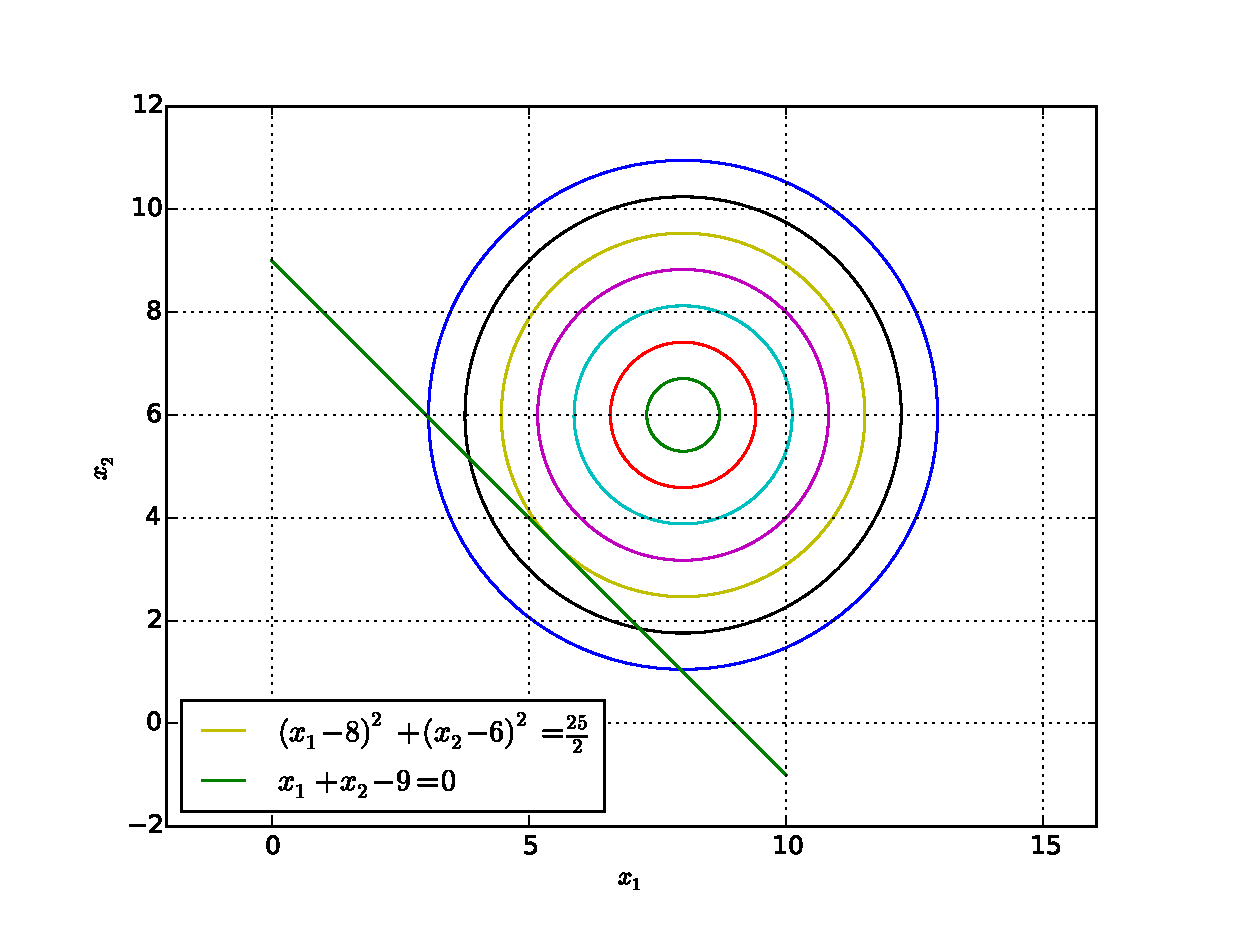
\includegraphics[width=\columnwidth]{./chapter2/figs/2.1.eps}
\caption{ Finding $ \displaystyle \min_{\mbf{x}}f\brak{\mbf{x}}$}.
\label{fig.2.1}	
\end{figure}
%
\begin{problem}
Obtain a theoretical solution for problem \ref{convex_code} using coordinate geometry.
\end{problem}
\solution 
From \eqref{eq2_1_line} and \eqref{eq2_1_circ}, 
%
\begin{align}
r^2 & = (x_1-8)^2 + (3- x_1)^2 \\
&= 2 x_1^2 - 22 x_1 + 73 \\
\Rightarrow r^2 &= \frac{\brak{2x_1-11}^2 + 5^2}{2}
\end{align}
%
which is minium when $x_1 = \frac{11}{2}, x_2 = \frac{7}{2}$.  The minimum value is $\frac{25}{2}$ and 
the radius $r = \frac{5}{\sqrt{2}}$.
\begin{problem}
\label{lagrange}
	Define 
	\begin{equation}
	\label{lagrangian}
	L\brak{\mbf{x},\lambda} = f\brak{\mbf{x}} - \lambda g\brak{\mbf{x}}%, \quad \lambda > 0
	\end{equation}
and
\begin{equation}
\nabla =  
\begin{pmatrix}
\frac{\partial}{\partial x_1} \\
\frac{\partial}{\partial x_2} \\
\frac{\partial}{\partial \lambda} 
\end{pmatrix}
\end{equation}
Solve the equations
%
\begin{align}
\nabla L\brak{\mbf{x},\lambda} &= 0.
\label{tangent}
\end{align}
%
How is this related to problem \ref{convex_code}? What is the sign of $\lambda$?  $L$ is known as the Lagrangian and the above technique is known as the Method of Lagrange Multipliers.
\end{problem}
\solution
From \eqref{eq2_1_line} and \eqref{eq2_1_circ}, 
%
\begin{align}
L\brak{\mbf{x},\lambda} &= (x_1-8)^2 + (x_2-6)^2 - \lambda \brak{x_1 + x_2 - 9} \\
\Rightarrow \nabla L\brak{\mbf{x},\lambda}  & = 
\begin{pmatrix}
2x_1  - 16 - \lambda \\
2x_2 - 12 - \lambda \\
x_1 + x_2 -9
\end{pmatrix}
\\
&=
\begin{pmatrix}
2 &0 & - 1 \\
0 &2 & - 1 \\
1 & 1 & 0 
\end{pmatrix}
\begin{pmatrix}
x_1 \\
x_2 \\
\lambda
\end{pmatrix}
= 
\begin{pmatrix}
16 \\
 12 \\
9
\end{pmatrix}
=
0 
\\
\Rightarrow 
\begin{pmatrix}
x_1 \\
x_2 \\
\lambda
\end{pmatrix}
&= 
\begin{pmatrix}
\frac{11}{2} \\
 \frac{7}{2} \\
-5
\end{pmatrix}
\end{align}
%
using the following python script.  Note that this method yields the same result as the previous exercises.  Thus, $\lambda$ is negative.
%	
\lstinputlisting{./chapter2/codes/2.3.py}
%
\begin{problem}
\label{ch2_constraint}
Modify the code in problem \ref{convex_code} to find a graphical solution for minimising
\begin{align}
f\brak{\mbf{x}} = (x_1-8)^2 + (x_2-6)^2
\end{align}
with constraint
\begin{align}
\label{convex-constraint}
g\brak{\mbf{x}} = x_1 + x_2 - 9 \geq 0
\end{align}
\end{problem}
\solution 
This problem reduces to finding the radius of the smallest circle in the shaded area in Fig. \ref{fig.2.4} .  It is clear that this radius is 0.
%	
\lstinputlisting{./chapter2/codes/2.4.py}
%
\begin{figure}[h]
\centering
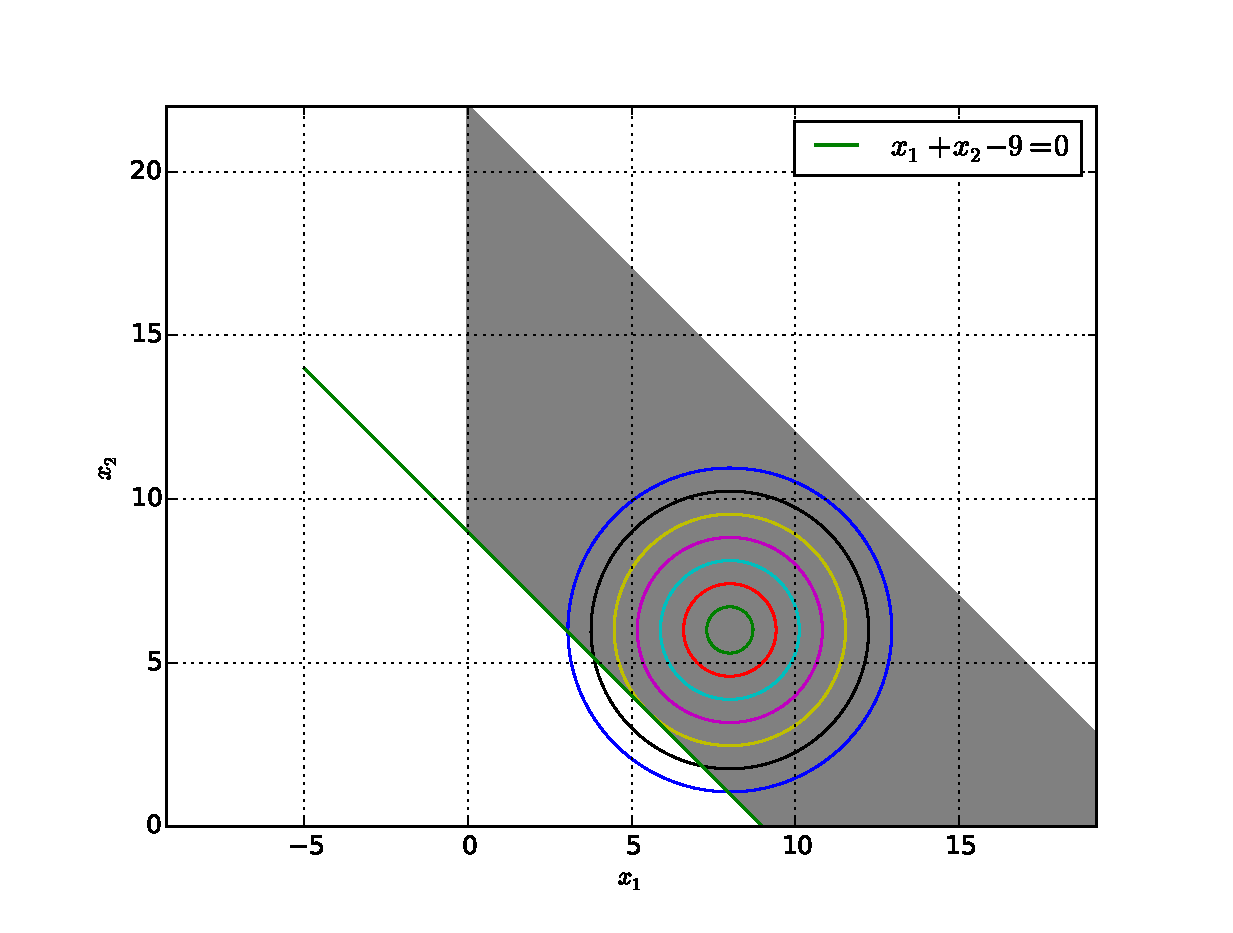
\includegraphics[width=\columnwidth]{./chapter2/figs/2.4.eps}
\caption{ Smallest circle in the shaded region is a point.}
\label{fig.2.4}	
\end{figure}
%
\begin{problem}
\label{ch2_lagrange_fail}
Now use the method of Lagrange multipliers to solve  problem \ref{ch2_constraint} and compare with the graphical solution.  Comment.
\end{problem}
%
\solution Using the method of Lagrange multipliers, the solution is the same as the one obtained in  problem \ref{ch2_constraint}, which is different from the graphical solution.  This means that the Lagrange multipliers method cannot be applied blindly.
\begin{problem}
Repeat problem \ref{ch2_lagrange_fail} by keeping 
 $\lambda=0$.   Comment.
\end{problem}
\solution Keeping $\lambda = 0$ results in $x_1 = 8, x_2 = 6$, which is the correct solution.  The minimum value of $f\brak{\mbf{x}}$ without any constraints lies in the region $g\brak{\mbf{x}} = 0$.  In this case, $\lambda = 0$.  
%
%
\begin{problem}
\label{ch2_constraint_border}
Find a graphical solution for minimising
\begin{align}
f\brak{\mbf{x}} = (x_1-8)^2 + (x_2-6)^2
\end{align}
with constraint
\begin{align}
\label{convex-constraint}
g\brak{\mbf{x}} = x_1 + x_2 - 9 \leq 0.
\end{align}
Summarize your observations.
\end{problem}
%
\solution In Fig. \ref{fig.2.7}, the shaded region represents the constraint.  Thus, the solution is the same as the one in problem \ref{ch2_constraint}. This implies that the method of
Lagrange multipliers can be used to solve the optimization problem with this inequality constraint as well.  Table \ref{table.2.7} summarizes the conditions for this based on the observations so far.
\lstinputlisting{./chapter2/codes/2.7.py}
%
\begin{figure}[h]
\centering
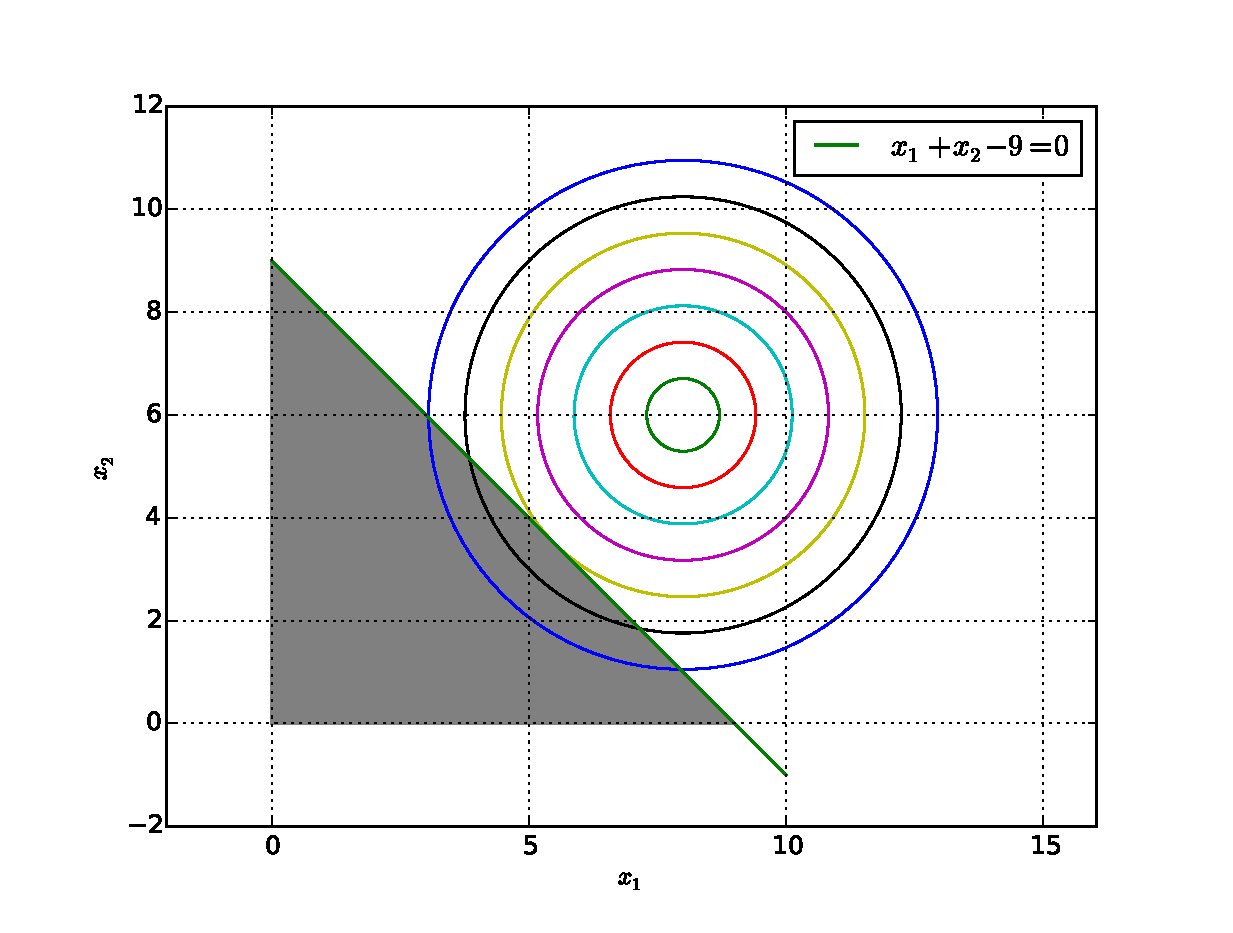
\includegraphics[width=\columnwidth]{./chapter2/figs/2.7.eps}
\caption{ Finding $ \displaystyle \min_{\mbf{x}}f\brak{\mbf{x}}$.}
\label{fig.2.7}	
\end{figure}
\input{./chapter2/figs/tab.2.7.tex}
%
\begin{problem}
\label{ch2_prob_upper}
Find a graphical solution for 	 
	 \begin{align}
	 \label{ch2_second_min}
	\min_{\mbf{x}} f\brak{\mbf{x}} = (x_1-8)^2 + (x_2-6)^2
	 \end{align}
	 with constraint
	 \begin{align}
	 \label{ch2_second_const}
	 g\brak{\mbf{x}} = x_1 + x_2 - 18 = 0
	 \end{align}
\end{problem}	 
%
\solution
%	
\lstinputlisting{./chapter2/codes/2.8.py}
%
\begin{figure}[h]
\centering
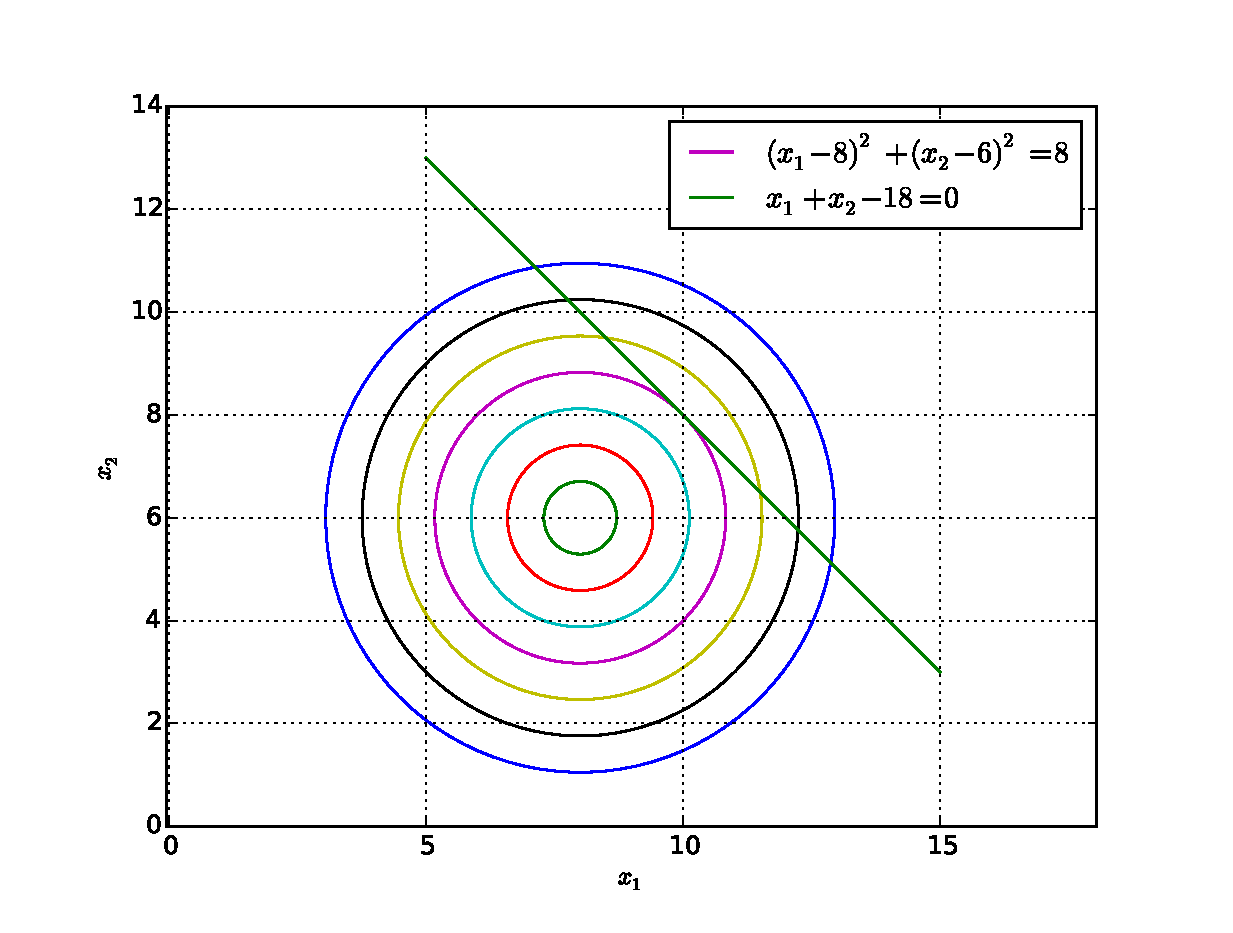
\includegraphics[width=\columnwidth]{./chapter2/figs/2.8.eps}
\caption{ Finding $ \displaystyle \min_{\mbf{x}}f\brak{\mbf{x}}$.}
\label{fig.2.8}	
\end{figure}
%
\begin{problem}
Repeat problem \ref{ch2_prob_upper} using the method of Lagrange mutipliers.  What is the sign of $\lambda$?
\end{problem}
%
\solution
From \eqref{ch2_second_min} and \eqref{ch2_second_min}, 
%
\begin{align}
L\brak{\mbf{x},\lambda} &= (x_1-8)^2 + (x_2-6)^2 - \lambda \brak{x_1 + x_2 - 18} \\
\Rightarrow \nabla L\brak{\mbf{x},\lambda}  & = 
\begin{pmatrix}
2x_1  - 16 - \lambda \\
2x_2 - 12 - \lambda \\
x_1 + x_2 -18
\end{pmatrix}
\\
&=
\begin{pmatrix}
2 &0 & - 1 \\
0 &2 & - 1 \\
1 & 1 & 0 
\end{pmatrix}
\begin{pmatrix}
x_1 \\
x_2 \\
\lambda
\end{pmatrix}
= 
\begin{pmatrix}
16 \\
 12 \\
18
\end{pmatrix}
=
0 
\\
\Rightarrow 
\begin{pmatrix}
x_1 \\
x_2 \\
\lambda
\end{pmatrix}
&= 
\begin{pmatrix}
10 \\
 8 \\
4
\end{pmatrix}
\end{align}
%
using the following python script.  Thus, $\lambda$ is positive and the minimum value of $f$ is 8.
%	
\lstinputlisting{./chapter2/codes/2.9.py}
%
%
\begin{problem}
\label{ch2_prob_upper_cond}
Solve
	 \begin{align}
	 \label{ch2_second_min}
	\min_{\mbf{x}} f\brak{\mbf{x}} = (x_1-8)^2 + (x_2-6)^2
	 \end{align}
	 with constraint
	 \begin{align}
	 \label{ch2_second_const}
	 g\brak{\mbf{x}} = x_1 + x_2 - 18 \geq 0 
	 \end{align}
\end{problem}	 
%
\solution Since the unconstrained solution is outside the region $g\brak{\mbf{x}} \geq 0$, the solution is the same as the one in problem \ref{ch2_prob_upper}.
%
\begin{problem}
Based on the problems so far, generalise the Lagrange multipliers method for 
%
	 \begin{align}
	 \label{ch2_lagrange_ineq}
	\min_{\mbf{x}} f\brak{\mbf{x}} , \quad 
	 g\brak{\mbf{x}}  \geq 0 
	 \end{align}
%
\end{problem}
%
\solution
Considering $L\brak{\mbf{x},\lambda} = f\brak{\mbf{x}} - \lambda g\brak{\mbf{x}}$, for $g\brak{\mbf{x}} = x_1 + x_2 - 18 \geq 0$ we found $\lambda > 0 $ and for $g\brak{\mbf{x}} = x_1 + x_2 - 9 \leq 0, \lambda < 0$. A single condition can be obtained by framing the optimization problem as
%
	 \begin{align}
	 \label{ch2_lagrange_ineq_summary}
	\min_{\mbf{x}} f\brak{\mbf{x}} , \quad 
	 g\brak{\mbf{x}}  \leq 0 
	 \end{align}
%
with the Lagrangian
%
\begin{equation}
%\label{ch2_kkt_necessary}
L\brak{\mbf{x},\lambda} = f\brak{\mbf{x}} + \lambda g\brak{\mbf{x}}, %\quad  \lambda > 0,  g\brak{\mbf{x}} \leq 0.
\end{equation}
%
provided
%
\begin{equation}
\label{ch2_kkt_necessary}
\nabla L\brak{\mbf{x},\lambda} = 0 \Rightarrow \lambda > 0
\end{equation}
else, $\lambda = 0$.
\begin{problem}
Solve
 \begin{align}
 \label{ch2_kkt_problem}
\min_{\mbf{x}} f\brak{\mbf{x}} = 4x_1^2 + 2x_2^2
 \end{align}
 with constraints
 \begin{align}
 g_1\brak{\mbf{x}} = 3x_1 + x_2-8 = 0\\
 g_2 \brak{\mbf{x}}= 15 - 2x_1 - 4x_2 \geq 0
 \end{align}
 \end{problem}
%
\solution Considering the Lagrangian
%
\begin{align}
L\brak{\mbf{x},\lambda} &= f\brak{\mbf{x}} + \lambda g_1\brak{\mbf{x}} - \mu g_2\brak{\mbf{x}} \\
 &= 4x_1^2 + 2x_2^2 + \lambda \brak{3x_1 + x_2-8} 
 \nonumber \\
 &\,-\mu\brak{15 - 2x_1 - 4x_2},\\
 \nabla L\brak{\mbf{x},\lambda}  & = 
\begin{pmatrix}
8x_1 + 3 \lambda  +2 \mu  \\
4x_2 + \lambda + 4 \mu \\
3x_1 + x_2 -8 \\
 - 2x_1 - 4x_2 + 15
\end{pmatrix}
= 0
\end{align}
%
resulting in the matrix equation
%
\begin{align}
\Rightarrow 
\begin{pmatrix}
8 &0 & 3 & 2\\
0 &4 & 1 & 4 \\
3 & 1 & 0 &0  \\
2 & 4 & 0 & 0
\end{pmatrix}
\begin{pmatrix}
x_1 \\
x_2 \\
\lambda
\\
\mu
\end{pmatrix}
&=
\begin{pmatrix}
0 \\
0 \\
8 \\
15
\end{pmatrix}
\\
\Rightarrow 
\begin{pmatrix}
x_1 \\
x_2 \\
\lambda
\\
\mu
\end{pmatrix}
&= 
\begin{pmatrix}
1.7 \\
 2.9 \\
-3.12 \\
-2.12
\end{pmatrix}
\end{align}
%
using the following python script.  The (incorrect) graphical solution is available in Fig. \ref{fig.2.12}
%	
\lstinputlisting{./chapter2/codes/2.12.py}
%
Note that $\mu < 0 $, contradicting the necessary condition in \eqref{ch2_kkt_necessary}. 
%
\begin{figure}[h]
\centering
\includegraphics[width=\columnwidth]{./chapter2/figs/2.12_1.eps}
\caption{ Incorrect solution is at intersection of all curves $r = 5.33$}
\label{fig.2.12}	
\end{figure}
\begin{problem}
Obtain the correct solution to the previous problem by considering $\mu = 0$.
\end{problem}
\begin{figure}[h]
\centering
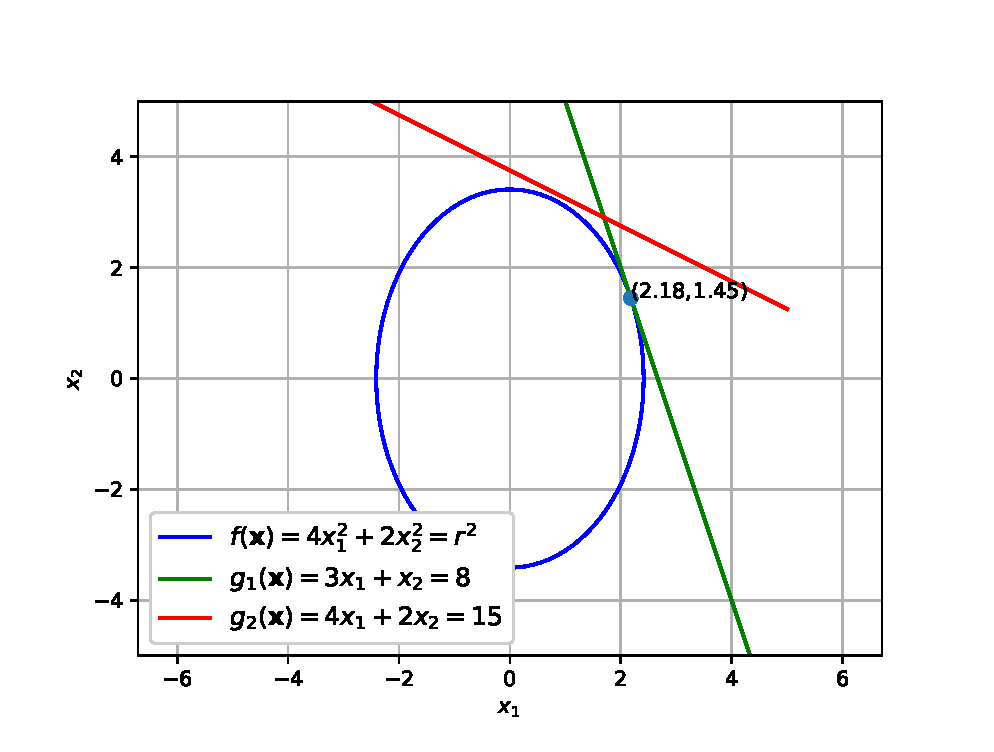
\includegraphics[width=\columnwidth]{./chapter2/figs/2.12_2.eps}
\caption{ Optimal solution is where $g_1(x)$ touches the curve $r = 4.82$}
\label{fig.2.13}	
\end{figure}
%
%
\begin{problem}
Solve
 \begin{align}
 \label{ch2_kkt_problem}
\min_{\mbf{x}} f\brak{\mbf{x}} = 4x_1^2 + 2x_2^2
 \end{align}
 with constraints
 \begin{align}
 g_1\brak{\mbf{x}} = 3x_1 + x_2-8 = 0\\
 g_2 \brak{\mbf{x}}= 15 - 2x_1 - 4x_2 \leq 0
 \end{align}
 \end{problem}
%
\begin{problem}
Based on whatever you have done so far,	list the steps that you would use in general for solving a convex optimization problem  like \eqref{ch2_kkt_problem}  using Lagrange Multipliers. 
These are called Karush-Kuhn-Tucker(KKT) conditions.
\end{problem}
\solution For a problem defined by 
\begin{align}
\mbf{x^*} &= \min_{\mbf{x}}f(\mbf{x})
\\
\text{subject to } h_i(\mbf{x}) &= 0, \forall i=1,..,m
\\
\text{subject to } g_i(\mbf{x}) &\le 0, \forall i=1,..,n
\end{align}
%
the optimal solution is obtained through
%
\begin{align}
\mbf{x^*} &= \min_{\mbf{x}}L(\mbf{x}, \mbf{\lambda}, \mbf{\mu}) 
\\
&= \min_{\mbf{x}}f(\mbf{x})  + \underset{i=1}{\overset{m}{\sum}} \lambda_i h_i(\mbf{x}) + \underset{i=1}{\overset{n}{\sum}} \mu_i g_i(\mbf{x}),
\end{align}
%
using the KKT conditions
%
\begin{align}
\Rightarrow \nabla_\mbf{x} f(\mbf{x})  + \underset{i=1}{\overset{m}{\sum}} \nabla_\mbf{x} \lambda_i h_i(\mbf{x}) + \underset{i=1}{\overset{n}{\sum}} \mu_i \nabla_\mbf{x} g_i(\mbf{x}) = 0 
\\
\text{subject to }\mu_i g_i(\mbf{x}) = 0, \forall i = 1,..,n
\\
\text{and }\mu_i \ge 0, \forall i = 1,..,n
\end{align}
%
\begin{problem}
	Maxmimize 
	%
	\begin{align}
	f(\mbf{x}) &= \sqrt{x_1x_2}
	\end{align}
	%
	with the constraints
	%
	\begin{align}
	x_1^2&+x_2^2 &\leq 5 \\
	x_1 \geq 0,& x_2 &\geq 0
	\end{align}
	%
\end{problem}
%
\begin{problem}
	\label{convex_sdp_eqiv}
	%
	Solve
	\begin{equation}
	\min_{\mbf{x}} \quad x_1 + x_2
	\end{equation}
	%	
	with the constraints
	\begin{equation}
	x_1^2 - x_1 + x_2^2 \leq 0
	\end{equation}
	%
where 
$
\mbf{x} = \begin{pmatrix}
x_1 \\
x_2
\end{pmatrix}
$
\end{problem}
\solution Using the method of Lagrange multipliers,
%
\begin{align}
\label{ch2_sd_kkt}
\nabla \cbrak{f(\mbf{x})  +  \mu g(\mbf{x}) }= 0 , \quad \mu \ge 0
\end{align}
%
resulting in the equations
%
\begin{align}
2x_1\mu -\mu + 1 &= 0 \\
2x_2\mu + 1 &=0 \\
x_1^2 -x_1 + x_2^2 &= 0 
\end{align}
%
which can be simplified to obtain 
%
\begin{align}
\brak{\frac{1-\mu}{2\mu}}^2 + \brak{\frac{1}{2\mu}}^2 + \frac{1-\mu}{2\mu} &= 0 \\
\Rightarrow 1 + \mu^2 -2\mu + 1 + 2\mu\brak{1-\mu} &= 0 \\
\Rightarrow \mu^2 =2, or \mu &= \pm \sqrt{2} 
\end{align}
%
From \eqref{ch2_kkt_problem},  $\mu \ge 0 \Rightarrow  \mu = \sqrt{2}$. The desired solution is
%
\begin{equation}
\mbf{x} = 
\begin{pmatrix}
 \frac{\sqrt{2}-1}{2\sqrt{2}} \\
-\frac{1}{2\sqrt{2}} 
\end{pmatrix}
\end{equation}
%
\\
{\em Graphical solution:} The constraint can be expressed as
%
\begin{align}
x_1^2 - x_1 + x_2^2 &\le 0 \\
\Rightarrow \brak{x_1 - \frac{1}{2}}^2 + x_2^2 & \le \brak{\frac{1}{2}}^2
\end{align}
%
%	
\lstinputlisting{./chapter2/codes/2.15.py}
%
%
\begin{figure}[h]
\centering
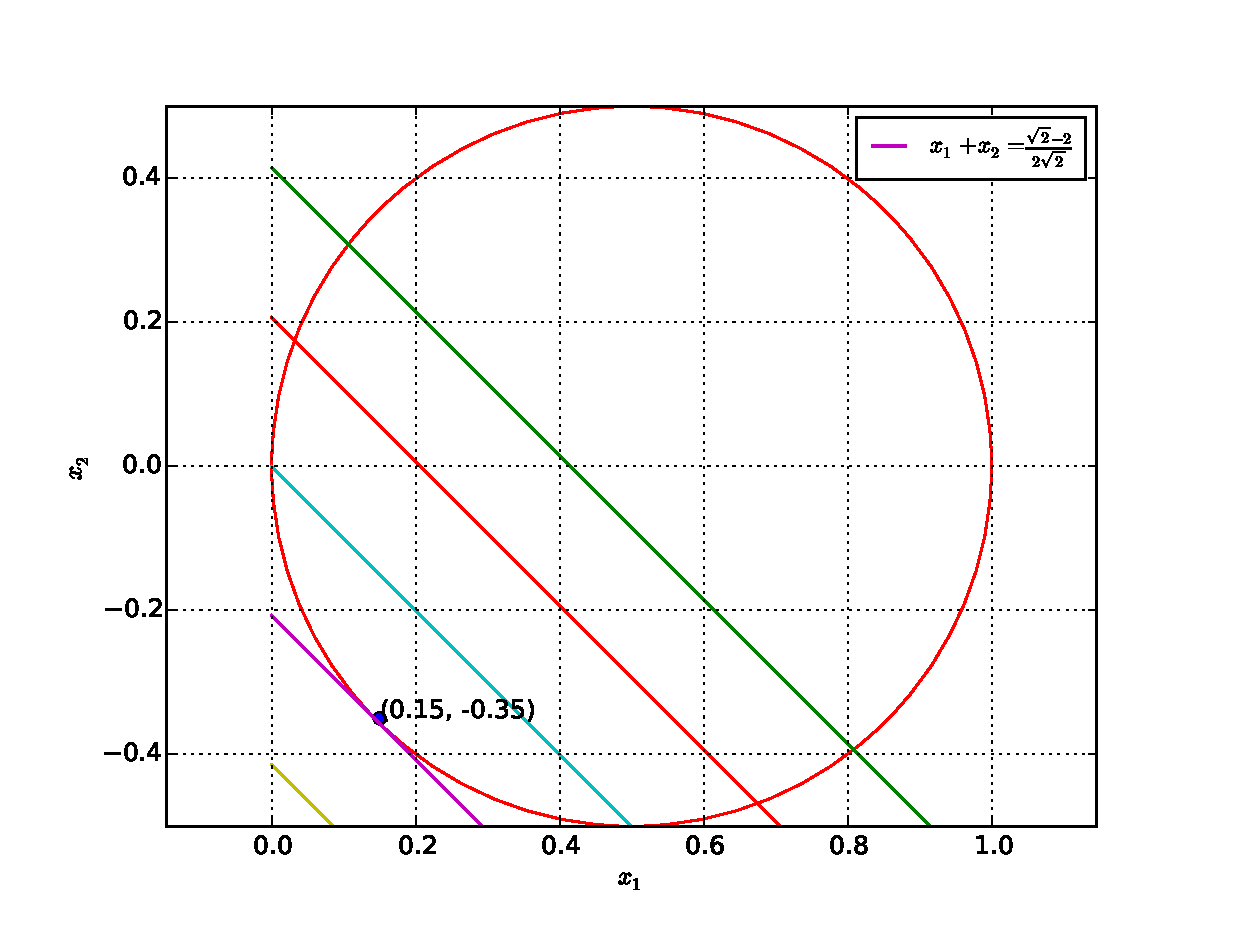
\includegraphics[width=\columnwidth]{./chapter2/figs/2.15.eps}
\caption{ Optimal solution is the lower tangent to the circle}
\label{fig.2.15}	
\end{figure}
%


